% Generated by benchmarks/make_tables.py -- do not edit by hand.
% Source runs:
%   app-uringpy-314r-20261006T193228Z: 150/150 runs ok, commit d9bc686, image sha256:197cfae00203
%   app-uringpy-314tr-20261006T212136Z: 120/120 runs ok, commit d9bc686, image sha256:e8775516edb3
%   baselines-uringpy-314-20261006T143743Z: 40/40 runs ok, commit b60fe24, image sha256:446f9f262d4f
%   batch-uringpy-314-20261006T123624Z: 30/30 runs ok, commit b60fe24, image sha256:446f9f262d4f
%   factorial-uringpy-314r-20261006T185824Z: 75/75 runs ok, commit d9bc686, image sha256:197cfae00203
%   handler-uringpy-314h-20261006T161108Z: 180/180 runs ok, commit 5b28fd1, image sha256:b48d32345e07
%   handler-uringpy-314h-20261006T173221Z: 60/60 runs ok, commit 5b28fd1, image sha256:b48d32345e07
%   handler-uringpy-314r-20261006T204033Z: 90/90 runs ok, commit d9bc686, image sha256:197cfae00203
%   handler-uringpy-314th-20261006T175923Z: 90/90 runs ok, commit 5b28fd1, image sha256:7894a7383a1b
%   scaling-uringpy-314-20261006T111536Z: 120/120 runs ok, commit b60fe24, image sha256:446f9f262d4f
%   scaling-uringpy-314t-20261006T131651Z: 120/120 runs ok, commit b60fe24, image sha256:3602f9e5eda6
%   size-uringpy-314r-20261006T221543Z: 60/60 runs ok, commit d9bc686, image sha256:197cfae00203
\begin{figure}[t]
\centering
\definecolor{sA}{HTML}{2A78D6}
\definecolor{sB}{HTML}{EB6834}
\definecolor{sC}{HTML}{1BAF7A}
\definecolor{ink}{HTML}{52514E}
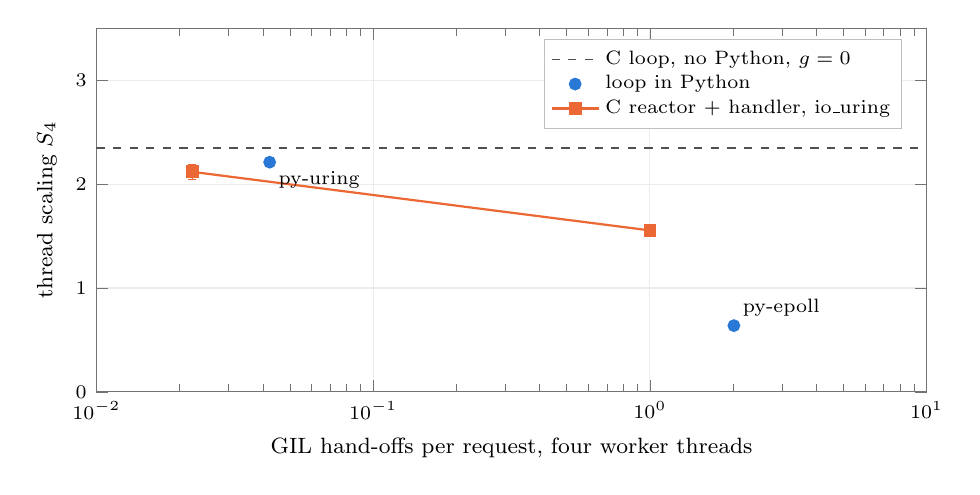
\begin{tikzpicture}
\begin{axis}[tick label style={font=\scriptsize}, label style={font=\footnotesize}, legend style={font=\scriptsize, draw=black!25, cells={anchor=west}, row sep=-1.5pt, inner sep=2pt}, grid=major, grid style={black!8}, axis line style={black!55}, tick style={black!55}, every axis plot/.append style={line width=0.8pt, mark size=1.9pt}, width=\columnwidth, height=62mm, xmode=log, xmin=0.01, xmax=10, ymin=0, ymax=3.5, xlabel={GIL hand-offs per request, four worker threads}, ylabel={thread scaling $S_4$}, legend pos=north east]
\addplot[ink, dashed, line width=0.6pt] coordinates {(0.01,2.345) (10,2.345)};
\addlegendentry{C loop, no Python, $g=0$}
\addplot[only marks, sA, mark=*, mark options={fill=sA}, error bars/.cd, y dir=both, y explicit, error bar style={line width=0.4pt}, error mark options={rotate=90, mark size=1.5pt, line width=0.4pt}] coordinates {(2.0121,0.63779) +- (0,0.01366) (0.042285,2.2107) +- (0,0.04391)};
\addlegendentry{loop in Python}
\addplot[sB, mark=square*, mark options={fill=sB}, error bars/.cd, y dir=both, y explicit, error bar style={line width=0.4pt}, error mark options={rotate=90, mark size=1.5pt, line width=0.4pt}] coordinates {(0.022199,2.1178) +- (0,0.07101) (1,1.554) +- (0,0.04147)};
\addlegendentry{C reactor + handler, \code{io\_uring}}
\node[font=\scriptsize, inner sep=3pt, anchor=south west] at (axis cs:2.0121,0.63779) {\code{py-epoll}};
\node[font=\scriptsize, inner sep=3pt, anchor=north west] at (axis cs:0.042285,2.2107) {\code{py-uring}};
\end{axis}
\end{tikzpicture}
\caption{Thread scaling at four workers against measured GIL hand-offs per request (GIL build; bars are 95\% half-widths). Loops in Python run the transport workload; the C reactors call the Python handler for every request, and the connected points are one reactor with the number of requests served per GIL acquisition varied. $^\ddagger$\,\code{py-uring-held} gives up the GIL as rarely as \code{py-uring} but holds it while the kernel performs the sends.}
\label{fig:handoffs}
\end{figure}
